\documentclass[a4paper,12pt]{article}
\usepackage[T1]{fontenc}
\usepackage[utf8]{inputenc}
\usepackage[italian]{babel}
\usepackage{lmodern}

\usepackage{enumitem}
\usepackage{commath}
\usepackage{bbold}
\usepackage{physics}
\usepackage{amsmath}
\usepackage{amsfonts}
\usepackage{amssymb}
\usepackage{amsthm}
\usepackage{graphicx}
\usepackage[colorinlistoftodos]{todonotes}
\PassOptionsToPackage{hyphens}{url}
\usepackage[colorlinks=true, allcolors=blue]{hyperref}
\usepackage{siunitx}
\sisetup{separate-uncertainty=true}
\usepackage{footnotebackref}
\usepackage{framed}
\usepackage{thmtools}
\usepackage{etoolbox}
\usepackage{fancybox}
\usepackage{slashed}
\newcommand{\DD}{\mathrm{D}}
\usepackage{mathrsfs}

\newenvironment{myleftbar}{%
\def\FrameCommand{\hspace{0.6em}\vrule width 2pt\hspace{0.6em}}%
\MakeFramed{\advance\hsize-\width \FrameRestore}}%
{\endMakeFramed}
\declaretheoremstyle[
spaceabove=6pt,
spacebelow=6pt
headfont=\normalfont\bfseries,
headpunct={} ,
headformat={\cornersize*{2pt}\ovalbox{\NAME~\NUMBER\ifstrequal{\NOTE}{}{\relax}{\NOTE}:}},
bodyfont=\normalfont,
]{exobreak}

\declaretheorem[style=exobreak, name=Esercizio,%
postheadhook=\leavevmode\myleftbar, %
prefoothook = \endmyleftbar]{exo}

\newcommand{\boxalign}[2][0.986\textwidth]{
  \par\noindent\tikzstyle{mybox} = [draw=black,inner sep=6pt]
  \begin{center}\begin{tikzpicture}
   \node [mybox] (box){%
    \begin{minipage}{#1}{\vspace{-5mm}#2}\end{minipage}
   };
\end{tikzpicture}\end{center}}

\usepackage{alumnistem}

\author{Jacopo Tissino}
\title{Soluzioni degli esercizi}
\date{Luglio 2020}

\usepackage[
backend=biber,
style=alphabetic,
sorting=nyt,
backref=true
]{biblatex}

\addbibresource{STEM_Indivisibility.bib}

% \title{L'indivisibilità del fotone: Summer STEM Academy 2020}

\begin{document}

\maketitle

\begin{exo}[Legge di Snell]
% Da impostare a lezione, senza finire il conto.
Consideriamo un'interfaccia fra due mezzi nei quali la luce si può trasmettere, ma con velocità diverse: definiamo l'\emph{indice di rifrazione} del mezzo, \(n\), il rapporto fra la velocità \(c\) della luce nel vuoto e la velocità \(v\) nel mezzo: \(n = c/v\).

Consideriamo un'onda piana incidente sulla barriera tale per cui l'angolo fra il vettore d'onda e la normale all'interfaccia sia \(\theta _{\text{in}}\). 
Chiamiamo \(\theta _{\text{out}}\) l'angolo fra la normale all'interfaccia e il vettore d'onda dell'onda uscente. 

I vettori d'onda entrante e uscente sono complanari, quindi il problema può essere trattato in due dimensioni.

Mostrare che vale la relazione 
%
\begin{align}
n _{\text{in}} \sin(\theta _{\text{in}}) = 
n _{\text{out}} \sin(\theta _{\text{out}})
\,.
\end{align}
\end{exo}

I fronti d'onda arrivano paralleli, il vettore d'onda ha un angolo \(\theta _{\text{in}}\) dalla normale. \(v = \lambda f\) deve valere sia dentro che fuori dal vetro: visto che \(f\) è la stessa (per continuità dei fronti all'interfaccia), abbiamo 
%
\begin{align}
    \frac{ \lambda _{\text{out}}}{\lambda _{\text{in}}} = \frac{n _{\text{in}}}{n _{\text{out}}}
    \,,
\end{align}
%
dove definiamo l'indice di rifrazione con \(v = c/n\). 
    
Se \(D\) è la distanza fra le creste misurata lungo l'interfaccia, abbiamo 
%
\begin{align}
    \frac{\lambda_{i}}{D} = \sin(\theta_{i})
    \,,
\end{align}
%
per \(i = \text{in}, \text{out}\). 
Da qui sostituendo si arriva direttamente all'espressione finale. 

\begin{exo}[Esperimento di Michelson, velocità della luce]

% Parametri: doppia distanza fra gli specchi \(D = \SI{3972.46}{ft}\), variazione lineare della posizione: \(d = \SI{114.85}{mm}\), raggio \(r = \SI{28.672}{feet}\), rivoluzioni al secondo: \(n = \SI{257.36}{Hz}\).

L'apparato che lo scienziato americano Michelson ha utilizzato nel 1880 \cite[]{michelsonExperimentalDeterminationVelocity1880} per determinare la velocità della luce permette una misura molto accurata.
La struttura dell'apparato è schematizzata in figura \ref{fig:michelson-apparatus}.
% Per una descrizione dell'apparato e una figura vedere Wikipedia \cite[figura 3]{wikipediacontributorsFizeauFoucaultApparatus2019}.
La luce parte dalla sorgente \(S\), rimbalza sullo specchio nel punto \(R\), va fino allo specchio \(M\) e torna indietro sui suoi passi.
Lo specchio mediano ruota attorno al punto \(R\), e la distanza fra il punto \(R\) e il punto \(M\) è molto grande.
In questo modo, nel tempo che la luce impiega per andare da uno specchio all'altro (e ritorno) lo specchio si è girato abbastanza affinché la luce non sia esattamente allineata con quella entrante. 
Misurando di quanto si sposta l'immagine della sorgente è possibile misurare la velocità di propagazione della luce.

Michelson ha ripetuto la misura innumerevoli volte, seguono i parametri ottenuti in una sola di queste misure: distanza fra gli specchi \(h = \SI{605}{m}\); variazione lineare della posizione (dal punto \(S\) al detector): \(d = \SI{115}{mm}\), raggio (dal punto \(R\) al punto \(S\)) \(r = \SI{8.74}{m}\); rivoluzioni al secondo dello specchio: \(n = \SI{257}{Hz}\).

I valori sono solo rappresentativi (per questo motivo ho anche troncato i decimali) e la stima di \(c\) che si ottiene non è ottima; quella conclusiva di Michelson invece è a solo \SI{.05}{\percent} di distanza dal valore correntemente accettato.

Qual'è la velocità della luce che avrebbe calcolato Michelson a partire dai dati precedentemente menzionati?

% Formula corretta: 
% %
% \begin{align}
% c _{\text{exp}} = \frac{2 \times 2 \pi \times 2 D n}{\arctan(d / r)} \approx \num{.994} c
% \,.
% \end{align}
\end{exo}

\begin{figure}[ht]
\centering
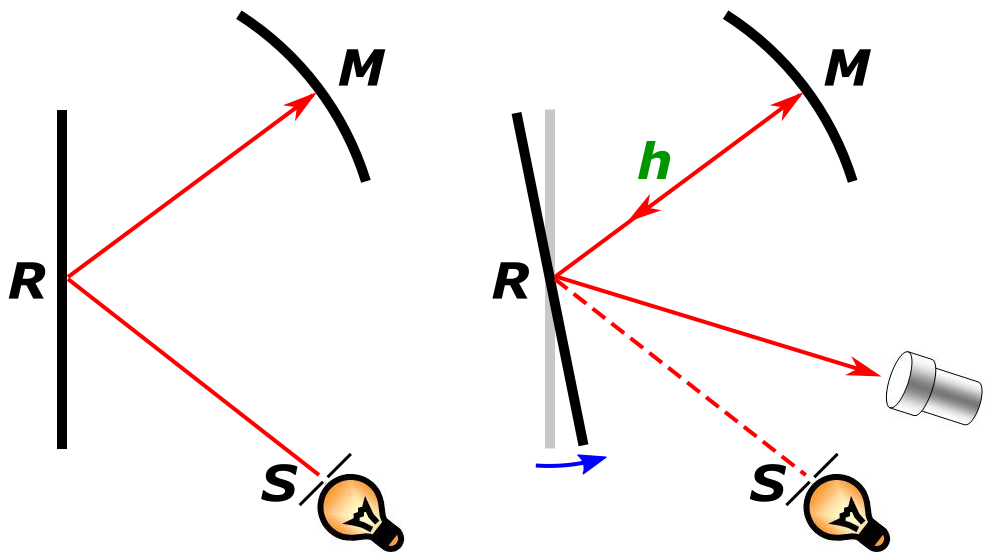
\includegraphics[width=\textwidth]{Speed_of_light_calculation_using_Foucault's_rotating_mirror.png}
\caption{Rappresentazione schematica dell'apparato di Michelson per le misurazione della velocità della luce \cite[]{aurantiacaSpeedLightCalculation2015}.
% \footnote{La figura è stata leggermente modificata al fine di non dare troppe informazioni. }
}
\label{fig:michelson-apparatus}
\end{figure}

La formula corretta è: 
%
\begin{align}
c _{\text{exp}} = \frac{2 \times 2 \pi \times 2 D n}{\arctan(d / r)} \approx \num{.994} c
\,.
\end{align}

\begin{exo}[Rate atteso di conteggi]
Il laser che useremo avrà una potenza di circa \SI{50}{mW} e la luce emessa avrà una lunghezza d'onda di circa \SI{500}{nm}. 

Mettiamo un filtro attenuatore che attenui la luce di un fattore 100, inoltre la SPDC capita solo a un fotone su \num{e7}.
La SPDC disperde le coppie entangled in un cono di apertura \SI{4}{\degree} circa, e dopo una distanza di \SI{50}{cm} circa alcuni di questi fotoni devono entrare in una fibra ottica di diametro circa \SI{100}{\micro m} per essere rilevati. 

Quant'è il numero di fotoni al secondo che ci aspettiamo di vedere nel gate, se il detector ha un'efficienza del \SI{10}{\percent}?
\end{exo}

Il rate atteso \(r\) è di:
%
\begin{align}
r = \frac{\SI{50}{mW}}{\hbar c / (\SI{500}{nm})}
\times 
\frac{\SI{100}{\micro m}}{\sin(\SI{4}{\degree}) \times 2 \pi  \times \SI{50}{cm}}
\times \num{e-7} \times \num{e-2} \times \num{e-1} \approx \SI{35}{kHz} 
\,.
\end{align}
%


\begin{exo}[Picchi delle differenze nei tempi]
    Dove ti aspetti che sia centrato il picco dei valori di \(t_R - t_G\)? E il picco di \(t_T - t_G\)? 
    % (Inserire foto dell'apparato con scala, in modo che si possano determinare i ritardi dovuti al tempo di viaggio della luce).
\end{exo}

\begin{figure}[ht]
\centering
\includegraphics[width=\textwidth]{single_photon_timedifferences}
\caption{Differenze temporali fra i conteggi dei fotoni in una ripetizione dell'esperimento descritto. In un colore più saturato sono rappresentati gli eventi contenuti entro 5 deviazioni standard dal picco della Gaussiana con la quale si possono fittare i dati.}
\label{fig:single_photon_timedifferences}
\end{figure}

\printbibliography

\end{document}
